\section{Design}

Tous les exercices ont été developpés en C++ en utilisant le paradigme de programmation objet et le design qui suit a été élaboré pour regrouper les différents composants de calculs. Néanmoins une recherche a été effectué pour determiner les limites de OpenMP et C++. Il semblerait que les conteneurs fournit par la STL\footnote{Standard Template Library : \url{http://www.sgi.com/tech/stl/}} ne soient pas threadsafe\footnote{On dit qu’un programme ou qu'une portion de code est thread-safe s'il fonctionne correctement durant une exécution simultanée par plusieurs threads (processus légers). \url{http://fr.wikipedia.org/wiki/Threadsafe}}. Une étude\footnote{C++ and OpenMP : \url{http://www.compunity.org/events/pastevents/parco07/parco_cpp_openmp.pdf}} donne une liste non-exaustive des précautions à prendre lors de l’utilisation de OpenMP en C++. Cependant la version OpenMP 3.0 apporte des concepts nouveaux permettant l’utilisation notemment des iterateurs. On peut ainsi, par exemple, s’affranchir de simple indexeur de tableau et étendre la parallelisation sur des listes chainées.

\subsection{Diagramme de classes}

\begin{figure}[here]
\centering
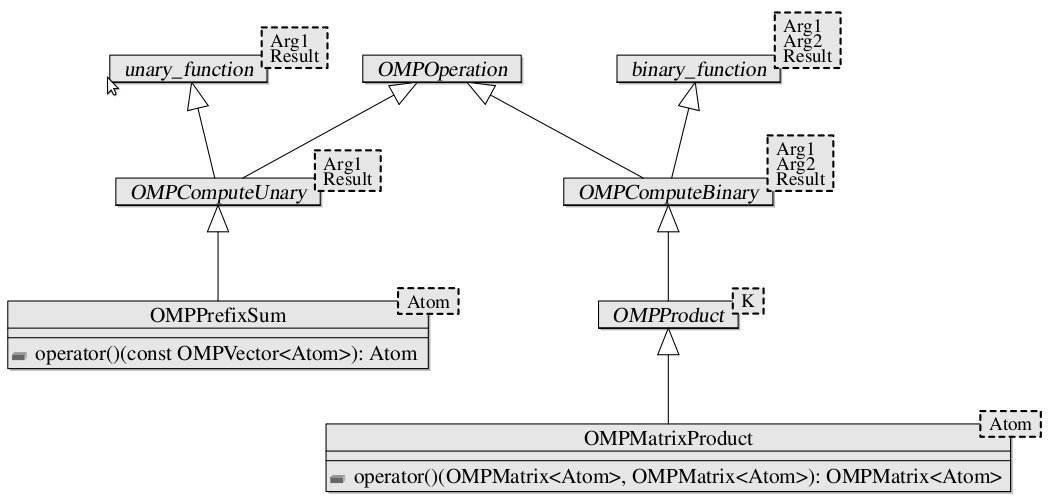
\includegraphics[scale=0.45]{diagram}
\caption{Diagramme de classes}
\label{fig:diagram}
\end{figure}

Deux grandes familles d'opérations coexistent. Elles sont présentées en figure \ref{fig:diagram}. Les opérations de calcul à paramètre unique ``OMPComputeUnary'' et celles à deux paramètres ``OMPComputeBinary''. Tous deux renvoient un résultat. Elles sont préfixées de ``OMP'' pour OpenMP\footnote{Open Multi-Processing : http://openmp.org/}. Le calcul de somme des prefixes prenant un seul paramètre en entrée ``OMPVector'' et renvoyant un ``Atom'', cette classe se situe dans la famille ``OMPComputeUnary''. Le produit matriciel se situe, quant à lui, dans la famille “OMPComputeBinary”, cette classe prend deux paramètres ``OMPMatrix'' et retourne le même type. On peut imaginer d'autres opérations comme, par exemple, un produit vectoriel.

\subsection{Surcharge d'opérateur}

Compte tenu des possibilités offertes par le langage C++, comme la surcharge des opérateurs, l'opérateur $*$ se voit ainsi surchargé dans la classe ``OMPMatrix'' afin d'appeler implicitement la classe ``OMPMatrixProduct'' pour le calcul du produit matriciel. Ainsi en écrivant le code $C = A * B$ ceci revient à écrire $C = OMPMatrixProduct()(A, B)$.
